\chapter{Financial market model\label{cha:chapter3}}
% input single, 0.3*np.sin(1.3 t) + N(0, 8)
% input signal 1.0*cos(0.1t) + N(0, 2) or N(0,1)}

% We deduce $0 < \alpha < \ln{(1 + \frac{1}{\delta})}$ since $\alpha, n > 0$. We should draw $\delta$ and $\alpha$ from gamma distribution carefully to make sure the constraints meet.
In this chapter, we formulate our financial market model by hysteretic operators, \textit{PI operator} and \textit{Presaich operator}, in detail and provide a practical way to generate synthetic data sets from this model. 

\section{Demand/Supply price formation\label{sec:chapter3:demand-supply-price-formation}}
We assume that the stock exchange accommodates three types of agents, which we call \textit{agents D}, \textit{agents N} and \textit{agents E}.

% \lackref{https://www.investopedia.com/terms/m/momentum_investing.asp}
\myupdate{The \textit{agents D} are used to describe the traders sell/buy stocks when the ratio of the price and a running maximum/minimum of the price  \footnote{The running maximum of the price means the maximum price the stock reached during the time frame $[s, t]$, where $s$ is the start time and t is the end of the time frame, and we denote it as $\max_{s \le \tau \le t} x(\tau)$. Similarly, the running minimum of price is the minimum price among the time frame $[s, t]$ and it's given by $\min_{s \le \tau \le t} x(\tau)$}  hits the given threshold. This strategy is a plausible pattern for an important subset of real-world traders | so-called momentum traders \lackref{} who believe that a stock that has performed well in the past tends to perform well in the future, and a stock that has performed poorly in the past tends to perform poorly in the future. Momentum traders seek stocks that are moving significantly in one direction and attempt to ride the momentum to obtain the desired profit. As a result, this strategy tends to exaggerate recent price movements, and induce, in a plausible manner, both the long-term mispricings and sudden reversals that are characteristic of financial systems.}    

% \lackref{https://www.investopedia.com/articles/trading/06/fundamentalapproach.asp}
\myupdate{The \textit{agents N} are used to describe the traders sell/buy stocks when the price of the stock is overvalued/undervalued. This strategy plays an important role in real-world traders | so-called fundamentalist traders, who use fundamental analysis to help predict the future value of the stocks. Fundamentalist traders analyze financial data to estimate a stock's intrinsic value. They believe a) if the stock's value is smaller than its intrinsic value, the price will go up and b) if the stock's value is higher than its intrinsic value, the price will go down.}

% \lackref{https://www.investopedia.com/articles/trading/02/100102.asp#different-types-of-traders}
\myupdate{The \textit{agents E} are used to described the traders | noise traders, whose decisions to buy or sell are irrational and erratic. The presence of noise traders in financial markets can then cause prices and risk levels to diverge from expected levels even if all other traders are rational.}

\myupdate{We consider K agents with the state $\chi_{k}=1$ of agent $k$ being either 1 or 0. The state $\chi_{k}=1$ indicates that the $k^{th}$ agent owns the stock and the $\chi_{k}=0$ means the agent doesn't own the stock. Furthermore,} 
We denote the price at time $n$ by $x_n$ \footnote{$x_n$ is log-price, which means $x_n = \ln p_n$, and $p_n$ is the original price observed in the real-world market.}, where time step $n=0, 1, 2, \ldots$. By definition, $x_n$ is the price of the transaction at time $n$. We will see below that demand equals supply at a time step $n$, but between any two consecutive time steps $n-1$ and $n$, there may occur numerous transactions until demand has become supply.

\begin{assumption}[Strategy of agents D \citep{dima2014}]\label{assumption:chapter3:strategy-of-agentD}
Agents D keep track of a trend (see \myfigref{fig:chapter3:strategy-illustration}). They buy stocks iff the price goes up and sell them iff the price goes down. The total amount of stocks that are in possession of all the agents D can be described as a Prandtl-Ishlinksii operator whose input is the price $x$. We denote this operator by
  $$P_D(x)$$
\end{assumption}
\begin{assumption}[Strategy of agents N]\label{assumption:chapter3:strategy-of-agentN}
The strategy of each of the agent N is characterized by a non-ideal relay with two fixed threshold $\alpha_L < \alpha_R$ (see \myfigref{fig:chapter3:strategy-illustration}). The relay is in state 0 if the price higher than $\alpha_R$ and in state 1 if the price is lower than $\alpha_L$. The agent buys one stock whenever his relay switches from 0 to 1 and sells one stock whenever his relay switches from 1 to 0. The total amount of stocks that are in possession of all the agents N can be described as a Preisach operator whose input is the price $x$. We denote this operator by
  $$P_N(x)$$
\end{assumption}

\begin{assumption}[Strategy of agents E]\label{assumpation:chapter3:strategy-of-agentE}
The strategy of each of agents E is used to break equilibrium in the market via buying or selling the additional stocks.
\end{assumption}

The following lemma is direct consequence of the definition of the operators $P_D(x)$ and $P_N(x)$.

\begin{lemma}\label{lemma:chapter3:reaction-to-price-change}
  \begin{enumerate}
    \item If $x$ is increasing, the $P_D(x)$ is increasing (agents D buy) and $P_N(x)$ is decreasing (agents N sell). 
    \item If $x$ is decreasing, the $P_D(x)$ is decreasing (agents D sell) and $P_N(x)$ is increasing (agents N buy).
  \end{enumerate}
\end{lemma}

\begin{remark}\label{remark:chapter3:1}
  Since $P_D(x)$ and $P_N(x)$ are not functions but operators, the monotone curves described in  \mylemmaref{lemma:chapter3:reaction-to-price-change} are not defined only by the current value of $x$, but \mydelete{depended}\myupdate{depend} on its prehistory.
\end{remark}

Denote $b_n$ the total amount of stocks that are in possession of all the agents D and N at time $n$. We will see below in \myassumptionref{assumption:chapter3:transitions-between-stabilized-prices} that $b_n$ may change as time goes on.

\begin{assumption}[Demand/supply price formation]\label{assumption:chapter3:demand/supply-price-formation}
At each moment $n$, the price $x_n$ is a stable solution of equation
\begin{equation}\label{eqn:chapter3:demand-supply-price-formation}
    P_D(x_{n}) + P_N(x_{n}) = b_{n}
\end{equation}
where the stability notion is explained in \myfigref{fig:chapter3:price-stability}, We will say that $x_n$ is a stabilized price.
\end{assumption}

\myupdate{We suppose that all agents D and agents N are at state $\chi=1$ (own the stocks) at the start time $s$ ($t_0$ in the \myfigref{fig:chapter3:strategy-illustration}) and we use log-price $x(t) = \ln p(t)$ instead of original price $p(t)$, $p(t)$ is the price we observe in the real market.
Considering the agent D, it tracks the price $x(t)$ and the running maximum $\max_{s \le \tau \le t} x(\tau)$. The agent D switches to state $\chi=0$ (sells the stock) at the first time $t > \tau$ when the inequality $\max_{s \le \tau \le t} x(\tau) - x(t) \ge \beta_R$ is satisfied for some threshold value $\beta_R > 0$. For example, if $\beta_R = 0.105$ then the agent D sells at the moment when the price drops from its peak value by 0.105 (or 10\% \footnote{The inequality $\max_{s \le \tau \le t} x(\tau) - x(t) \ge \beta_R$ is equivalent to $\ln \frac{\max_{s \le \tau \le t} p(\tau)}{p(t)} \ge \ln s = \beta_R$. By solving equation $\ln s = \beta_R$, we obtain $s \approx 1.11$ (or $\frac{10}{9}$), which means the original price drops from its peak value by 10\%.} in the original price scale). So the selling condition of agent D is $\theta := \min\{t > \tau : \max_{s \le \tau \le t} x(\tau) - x(t) \ge \beta_R \}$. This agent D adopts a similar strategy for deciding when to buy a stock again. The agent D tracks a threshold $x(t) - \min_{\theta \le \tau \le t} x(\tau) \ge \beta_L$ and switches back to state $\chi=1$ when it exceeds a value $\beta_L > 0$. Considering the agent N, it also tracks the price $x(t)$ and the running maximum $\max_{s \le \tau \le t} x(\tau)$. However, the agent N switches to state $\chi=0$ (sells the stock) at the first time  $t > \tau$ when the inequality $\max_{s \le \tau \le t} x(\tau) \ge \alpha_R$. We set the selling condition of agent N $\theta := \min\{ t > \tau : \max_{s \le \tau \le t} x(\tau) \ge \alpha_R \}$. Similarly, the agent N switches back to $\chi=1$ (buys a stock) again when $\min_{\theta \le \tau \le t} \le \alpha_L$.}

\begin{figure}[htb!]
    \centering
    % \subfloat[]{
        \scalebox{0.8}[0.7] {
            \documentclass{standalone}
\usepackage{pgfplots}
\pgfplotsset{compat=1.11}
\begin{document}
% Place the TikZ picture in a figure environment.
%\begin{figure}[htb]
% h: here, t: top, b: bottom, p: page of float
%% https://tex.stackexchange.com/questions/39017/how-to-influence-the-position-of-float-environments-like-figure-and-table-in-lat
%% ! indicates that some restrictions should be ignored (discussed later)
%% h indicates that the float is allowed to be placed inline
%% t indicates that the float is allowed to go into a top area
%% b indicates that the float is allowed to go into a bottom area
%% p indicates the the float is allowed to go on a float page or column area

    \begin{tikzpicture}[font=\small]
        \begin{axis} [
            height=10cm, width=20cm,
            xmin=-1, xmax=13, ymin=-0.2, ymax=1.5,
            xlabel={$t$},
            ylabel={$x(t)$},
                        % xtick={-2,-1.5,...,2}, ytick={-2,-1.5,...,2},
            xticklabel style={font=\tiny, xshift=0.5ex},
            yticklabel style={font=\tiny, yshift=0.5ex},
            axis line style={->},
            axis x line=middle,
            axis y line=middle,
            ticks=none,
            %grid=both,
           % legend pos=north west,
           legend style={at={(0.05,0.8)},anchor=south west}
        ]
        \draw[black, thick] plot [smooth,samples=200, tension=1] coordinates {(0,0) (1,0.97) (2,0.78) (3, 0.9) (4, 0.83) (5,1.1) (5.5, 1) (6.4,1.2) (7,0.3) (8,0.4) (9,0.2) (10,0.45) (11, 1.02)};

        % \draw [-,thick,blue] (4.3,0.9) -- (4.5,0.9);
        % \node[left] at (0,0.9) {$\beta$};
        \draw [dashed,blue] (0,0.92) -- (11,0.92);
        \node[left] at (0,0.92) {$\alpha_R$};
        \draw [dashed,red] (0,0.3) -- (11,0.3);
        \node[left] at (0,0.3) {$\alpha_L$};
            %%%%%%%%%%%%%%%%%%%%%%%%%%%%%%%%%%%%%%%%%%%%%%%%%%%%        


        \draw [dashed,green] (6,1.26) -- (7.5,1.26);
        \draw [dashed,green] (6,0.75) -- (7.5,0.75);
        
        \draw [solid,green,->] (7,1.26) -- (7,0.75);
        \draw [solid,green,->] (7,0.75) -- (7,1.26);
        \node[right] at (7,1.0) {$\beta_R$};


        \draw [dashed,green] (8.5,0.2) -- (10.5,0.2);
        \draw [dashed,green] (8.5,0.55) -- (10.5,0.55);
        
        \draw [solid,green,->] (9.5,0.2) -- (9.5,0.55);
        \draw [solid,green,->] (9.5,0.55) -- (9.5,0.2);
        \node[left] at (9.5,0.45) {$\beta_L$};
        
        %\node[left] at (0,0.92) {$\beta$};
        % \draw [dashed,green] (6,0.75) -- (7.5,0.75);

        \node[above left] at (0.,0.) {$O$};
        \node[above] at (7.1,0.3) {$M$};
        \node[above] at (7.75,0.29) {$N$};

        %%%%%%%%%%%%%%%%%%%%%%%%%%%%%%%%%%%%%%%%%%%%%%%%%%%%        
        \draw [dashed,black] (0.8,0.85) -- (0.8,0);
        \node[below] at (0.85,0) {$t_0$};
        \node[above left] at (0.85,0.85) {$A$};

        \draw [dashed,black] (1.24,1.01) -- (1.24,0);
        \node[below] at (1.24,0) {$t_1$};
        \node[above] at (1.24,1.01) {$B$};
        
        \draw [dashed,black] (2.1,0.78) -- (2.1,0);
        \node[below] at (2.1,0) {$t_2$};        
        \node[above] at  (2.1,0.78) {$C$};

        \draw [dashed,black] (3.1,0.9) -- (3.1,0);
        \node[below] at (3.1,0) {$t_3$};          
        \node[above] at  (3.1,0.9) {$D$};

        \draw [dashed,black] (3.8,0.82) -- (3.8,0);
        \node[below] at (3.8,0) {$t_4$};           
        \node[above] at  (3.8,0.82) {$E$};


        \draw [dashed,black] (5.1,1.1) -- (5.1,0);
        \node[below] at (5.1,0) {$t_5$};  
        \node[above] at  (5.1,1.1) {$F$};

        
        \draw [dashed,black] (5.5,1.) -- (5.5,0);
        \node[below] at (5.5,0) {$t_6$}; 
        \node[above] at  (5.5,1.)  {$G$};
        
        \draw [dashed,black] (6.2,1.23) -- (6.2,0);
        \node[below] at (6.2,0) {$t_7$}; 
        \node[above] at (6.2,1.24) {$H$};
        
        \draw [dashed,black] (7.2,0.21) -- (7.2,0);
        \node[below] at (7.2,0) {$t_8$};   
        \node[above] at (7.25,0.22) {$I$};
        
        \draw [dashed,black] (8,0.4) -- (8,0);
        \node[below] at (8.0,0) {$t_9$};  
        \node[above] at   (8,0.4)  {$J$};
        

        \draw [dashed,black] (9,0.2) -- (9,0);
        \node[below] at (9,0) {$t_{10}$};          
        \node[above] at  (9,0.2) {$K$};


        \draw [dashed,black] (9.9,0.44) -- (9.9,0);
        \node[below] at (9.9,0) {$t_{11}$};         
        \node[above] at (9.9,0.44) {$L$};

        \draw [dashed,black] (11,1.0) -- (11,0);
        \node[below] at (11,0) {$t_{12}$};         
        \node[above] at (11,1.0) {$Q$};        
        
        % \draw [-,thick,red] (4.35,0.59) -- (4.5,0.675);

        % \node[below] at (9.6,-0.036) {\Large$x_n$};
        % \node[below] at (1.6,-0.036) {\Large$x_{n-1}$};
    
        \end{axis}
    \end{tikzpicture}

\end{document}
        }
    % }
    \caption{Illustration strategy of agents D and agents N (see \mytableref{tbl:appendix:illustration-strategy-D,tbl:appendix:illustration-strategy-N} for details.)}
    \label{fig:chapter3:strategy-illustration}
    
\end{figure}

\begin{figure}[htb!]
    \centering
    \subfloat[Curves for growing price (stable equilibrium)]{
        \scalebox{1}[0.7] {
        \input{./tikz/market-price-equilibrium-stable-rise}
        }
        \label{fig:chapter3:rise-stable}
    }
    \subfloat[Curves for decaying price (stable equilibrium)]{
        \scalebox{1}[0.7] {
        \input{./tikz/market-price-equilibrium-stable-drop}
        }
        \label{fig:chapter3:drop-stable}
    }
    \hfill
    \subfloat[Curves for growing price (unstable equilibrium)]{
        \scalebox{1}[0.7] {
           \input{./tikz/market-price-equilibrium-unstable-rise-1}
        }
        \label{fig:chapter3:rise-unstable-1}
    }
    \subfloat[Curves for decaying price (unstable equilibrium)] {
        \scalebox{1}[0.7] {
        \input{./tikz/market-price-equilibrium-unstable-drop-1}
        }
        \label{fig:chapter3:drop-unstable-1}
    }
    \hfill
        \subfloat[Curves for growing price (unstable equilibrium)]{
        \scalebox{1}[0.7] {
        \input{./tikz/market-price-equilibrium-unstable-rise-2}
        }
        \label{fig:chapter3:rise-unstable-2}
    }
    \subfloat[Curves for decaying price (unstable equilibrium)] {
        \scalebox{1}[0.7] {
        \documentclass{standalone}
\usepackage{pgfplots}
\pgfplotsset{compat=1.11}
\begin{document}
% Place the TikZ picture in a figure environment.
%\begin{figure}[htb]
% h: here, t: top, b: bottom, p: page of float
%% https://tex.stackexchange.com/questions/39017/how-to-influence-the-position-of-float-environments-like-figure-and-table-in-lat
%% ! indicates that some restrictions should be ignored (discussed later)
%% h indicates that the float is allowed to be placed inline
%% t indicates that the float is allowed to go into a top area
%% b indicates that the float is allowed to go into a bottom area
%% p indicates the the float is allowed to go on a float page or column area

    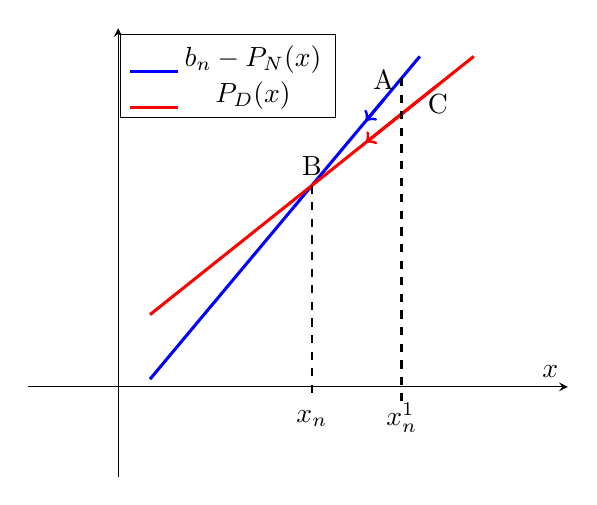
\begin{tikzpicture}
        \begin{axis} [
            xmin=-0.5, xmax=2.5, ymin=-0.5, ymax=2, 
            xlabel={$x$},
            % xtick={-2,-1.5,...,2}, ytick={-2,-1.5,...,2},
            xticklabel style={font=\tiny, xshift=0.5ex},
            yticklabel style={font=\tiny, yshift=0.5ex},
            axis line style={->},
            axis x line=middle,
            axis y line=middle,
           % legend pos=north west,
           ticks=none,
           legend style={at={(0.17,0.8)},anchor=south west}
        ]
        % \addplot+[mark=none, line width=1.1, color=blue, domain=-2:-0.5] {x+0.5};
        % \addplot+[mark=none, line width=1.1, color=blue, domain=-0.5:0.5] {0};
        \addplot+[mark=none, line width=1.1, color=blue, domain=0.1:1.6][xshift=5pt,yshift=-5pt] {1.2*x};
        
        \addplot+[mark=none, line width=1.1, color=red, domain=0.1:1.9][xshift=5pt,yshift=-5pt] {0.8*x + 0.4};
        % \addlegendentry{$k=1$}
        
        % \node[below] (A) at (0.3, 0.36) {A};
         \node[below][xshift=5pt,yshift=-5pt] (C) at (1.7, 1.76) {C};
        
        \node[above][xshift=5pt,yshift=-5pt] (B) at (1, 1.2) {B};
        % \node[above] (C) at (0.3, 0.64) {C};
        \node[above][xshift=5pt,yshift=-5pt] (A) at (1.4, 1.68) {A};
        \node[below][xshift=5pt,yshift=-5pt] (xn) at (1.5, 0.04) {$x^{1}_n$};
    \node[below][xshift=5pt,yshift=-5pt] (xn) at (1, 0) {$x_n$};

        % \node[below] (PD) at (1.7, 1.76) {$P_D$};
        % \node[above] (PN) at (1.4, 1.68) {$P_N$};

        % \addplot[->,line width=1.1,color=blue] coordinates {(0.3, 0.36)  (0.7, 0.84)};
        % \addplot[->,line width=1.1,color=red] coordinates {(0.3, 0.64)  (0.7, 0.96)};

        \addplot[->,line width=1.1,color=red][xshift=5pt,yshift=-5pt] coordinates {(1.7, 1.76)  (1.3, 1.44)};
        \addplot[->,line width=1.1,color=blue][xshift=5pt,yshift=-5pt] coordinates {(1.4,1.68)  (1.3, 1.56)};

        \addplot[dashed,line width=1, color=black][xshift=5pt,yshift=-5pt] coordinates {(1, 1.2)  (1,0)};
        \addplot[dashed,line width=1, color=black][xshift=5pt,yshift=-5pt] coordinates {(1.5, 1.8)  (1.5,0)};

        \addlegendentry{$b_n - P_N(x)$}
        \addlegendentry{$P_D(x)$}

        \end{axis}
    \end{tikzpicture}

\end{document}
        }
        \label{fig:chapter3:drop-unstable-2}
    }
    \hfill
    \caption{Stability of solutions of \myformularef{eqn:chapter3:demand-supply-price-formation}.     \myfigref{fig:chapter3:rise-stable,fig:chapter3:rise-unstable-1,fig:chapter3:rise-unstable-2} indicate \textit{agents D} buy stocks and \textit{agents N} sell stocks. \myfigref{fig:chapter3:drop-stable,fig:chapter3:drop-unstable-1,fig:chapter3:drop-unstable-2} imply \textit{agents D} is selling stocks and \textit{agents N} is buying stocks. 
    $x_n$ is the stable solution (price) for time step $n$. $x^{1}_n$ and $x^{2}_n$ in \myfigref{fig:chapter3:rise-unstable-1,fig:chapter3:rise-unstable-2,fig:chapter3:drop-unstable-1,fig:chapter3:drop-unstable-2} are the intermediate price during transaction.
    The difference between the equilibrium of (\myfigref{fig:chapter3:rise-unstable-1,fig:chapter3:drop-unstable-1}) and (\myfigref{fig:chapter3:rise-unstable-2,fig:chapter3:drop-unstable-2}) is that the price would grow in (\myfigref{fig:chapter3:rise-unstable-1,fig:chapter3:drop-unstable-1}) but decay in (\myfigref{fig:chapter3:rise-unstable-2,fig:chapter3:drop-unstable-2}).    
    }
    \label{fig:chapter3:price-stability}
\end{figure}
%\FloatBarrier

To explain how a stabilized price moves from \myupdate{one} equilibrium to the subsequent \mydelete{value}\myupdate{one}, we make the following assumption.

\begin{assumption}[Transitions between stabilized prices]\label{assumption:chapter3:transitions-between-stabilized-prices} 
  Suppose $x_{n-1}$ is a stabilized price as time $n-1$. In particular, it is a stable solution of equation
  \begin{equation}\label{eqn:chapter3:stable-price-eqn}
    P_D(x_{n-1}) + P_N(x_{n-1}) = b_{n-1}
  \end{equation}
  We assume that between time moments $n-1$ and $n$, some external agents E buy or sell some stocks. As a result, the total number of stocks that is in possession of agents D and N becomes $b_n$. Moreover, we assume that external agents do not stay at the stock exchange, i.e., the operators (their densities) $P_D(x)$ and $P_N(x)$ do not change in time.
  
  If $b_n \le b_{n-1}$, then external agents E buy $|b_{n}-b_{n-1}|$ stocks, which makes the price rise. As a result, agents D also buy. All the stocks bought by agents E and D are sold by agents N. This leads to the increase of the price to a new value $x_n^1$, where $x_n^1$ is the smallest solution of the equation
  \begin{equation}\label{eqn:chapter3:new-stable-price-eqn}
    P_D(x_n^1) + P_N(x_n^1) = b_n
  \end{equation}
  satisfying the inequality
  \begin{equation}
    x_n^1 > x_{n-1}
  \end{equation}

\mydelete{Note that small values $|b_n - b_{n-1}|$ may correspond to small change of the price as in \myfigref{fig:chapter3:price-change-without-bifurcation,fig:chapter5:dynamics-of-agents-1} or large changes as in \myfigref{fig:chapter3:price-change-with-bifurcation,fig:chapter5:dynamics-of-agents-2}. In the latter case, the price jumps up due to the fold bifurcation.}
\myupdate{  Note that small values $|b_n - b_{n-1}|$ may correspond to small change of the price as in \myfigref{fig:chapter3:price-change-without-bifurcation,fig:chapter5:dynamics-of-agents-1} or large changes as in \myfigref{fig:chapter3:price-change-bifurcation,fig:chapter5:dynamics-of-agents-2}. In the latter case, the price jumps up due to the fold bifurcation.}

  If $x_n^1$ is a stable \myupdate{solution} of \myformularef{eqn:chapter3:new-stable-price-eqn}, then, by definition, it coincides with the new stabilized price:
  \begin{equation}\label{eqn:new-price}
    x_n := x_n^1
  \end{equation}
  Otherwise, the price makes several jumps taking semi-stable values $x_n^2, \ldots, x_n^{m-1}$ and a stable value $x_n^m$ \mydelete{(hopefully with a finite m)} such that
%   \begin{equation}
%     x_{n}^1 > x_{n}^2, \quad x_{n}^3 > x_{n}^2, \quad x_{n}^3 > x_{n}^4,\quad x_{n}^{5} > x_{n}^4, \ldots
%   \end{equation}
  \begin{eqnarray*}
    P_D(x_{n}^1) &>& b_n - P_N(x_{n}^1),\quad x_n^1 > x_{n-1} \\ 
    P_D(x_{n}^2) &<& b_n - P_N(x_{n}^2),\quad x_{n-1} < x_n^2 < x_{n}^1 \\
    P_D(x_{n}^3) &>& b_n - P_N(x_{n}^3),\quad x_n^1 > x_n^3 > x_{n}^2 \\
   P_D(x_{n}^4) &<& b_n - P_N(x_{n}^4),\quad x_n^2 < x_n^4 < x_{n}^3 \\    
    &\ldots&   \\
    P_D(x_{n}^m) &=& b_n - P_N(x_{n}^m) 
  \end{eqnarray*}
  By definition, we set
  \begin{equation}
    x_n := x_n^m
  \end{equation}
  Analogously, the price will leave the stable value $x_{n-1}$ if $b_n > b_{n-1}$. In this case external agents E sell $b_n - b_{n-1}$ stocks, which decreases the price. As a result, agents D also sell. All the stocks sold by agents E and D are bought by agents N.
\end{assumption}

\begin{figure}[htb!]
 \subfloat[Price $x_{n-1}$ gets destabilized and increases without bifurcation)]{
    \scalebox{0.8}[0.7] {
        \documentclass{standalone}
\usepackage{pgfplots}
\pgfplotsset{compat=1.11}
\begin{document}
% Place the TikZ picture in a figure environment.
%\begin{figure}[htb]
% h: here, t: top, b: bottom, p: page of float
%% https://tex.stackexchange.com/questions/39017/how-to-influence-the-position-of-float-environments-like-figure-and-table-in-lat
%% ! indicates that some restrictions should be ignored (discussed later)
%% h indicates that the float is allowed to be placed inline
%% t indicates that the float is allowed to go into a top area
%% b indicates that the float is allowed to go into a bottom area
%% p indicates the the float is allowed to go on a float page or column area

    \begin{tikzpicture}
        \begin{axis} [
            height=10cm, width=20cm,
            xmin=-0.2, xmax=11, ymin=-0.2, ymax=1.5,
            xlabel={$x$},
                        % xtick={-2,-1.5,...,2}, ytick={-2,-1.5,...,2},
            xticklabel style={font=\tiny, xshift=0.5ex},
            yticklabel style={font=\tiny, yshift=0.5ex},
            axis line style={->},
            axis x line=middle,
            axis y line=middle,
            ticks=none,
            % grid=both,
           % legend pos=north west,
           legend style={at={(0.05,0.8)},anchor=south west}
        ]
         \draw [red,thick] plot [smooth,samples=200, tension=0.5] coordinates {(0.2,0.2) (1.8,0.55) (4, 0.61) (6, 0.8) (7,1.0) (8,1.15) (9.8,1.18) (10.5,1.2)};

        \addlegendimage{line width=0.3mm,color=red}
        \addlegendentry{$P_D(x)$}
   
        \draw [blue,thick] plot [smooth,samples=200, tension=0.5] coordinates { 
        (0.8,0.2) (1.5,0.5) (3,0.8) (6,0.85) (8,0.9) (9.8, 1.23) (10.5,1.33)};

        \addlegendimage{line width=0.3mm,color=blue}
        \addlegendentry{$b_{n-1} - P_N(x)$}
        
        \draw [dashed,blue,thick][xshift=10pt,yshift=-20pt] plot [smooth,samples=200, tension=0.5] coordinates { 
        (0.8,0.2) (1.5,0.5) (3,0.8) (6,0.85) (8,0.9) (9.8, 1.23) (10.5,1.33)};
        
        \addlegendimage{line width=0.3mm,color=blue,dashed}
        \addlegendentry{$b_{n} - P_N(x)$}

        \addplot[-,line width=1,color=black,dashed] coordinates {(1.5,0.50)  (1.5,0.)};
        \addplot[-,line width=1,color=black,dashed] coordinates {(2.7,0.578)  (2.7,0.)}; 

        \draw [-,thick,blue] (4.3,0.79) -- (4.5,0.832);
        \draw [-,thick,blue] (4.3,0.87) -- (4.5,0.832);

 
        \draw [-,thick,blue][xshift=10pt,yshift=-20pt]  (4.3,0.79) -- (4.5,0.832);
        \draw [-,thick,blue][xshift=10pt,yshift=-20pt]  (4.3,0.87) -- (4.5,0.832);

        \draw [-,thick,red] (4.3,0.67) -- (4.5,0.65);
        \draw [-,thick,red] (4.35,0.60) -- (4.5,0.65);
        
        \node[left] at (1.6,0.55) {$A$};
        \node[above] at (2.7,0.60) { $B$};
        % \node[below] at (3.2,0.0) {\Large$x^{intermediate}_n$};
        \node[below] at (2.7,-0.036) {\Large$x_n$};
        \node[below] at (1.6,-0.036) {\Large$x_{n-1}$};
    
        \end{axis}
    \end{tikzpicture}

\end{document}
        }
        \label{fig:chapter3:price-change-without-bifurcation}
    }
    \hfill
    \subfloat[Price $x_{n-1}$ gets destabilized and increases with fold bifurcation]{
    \scalebox{0.8}[0.7] {
        \documentclass{standalone}
\usepackage{pgfplots}
\pgfplotsset{compat=1.11}
\begin{document}
% Place the TikZ picture in a figure environment.
%\begin{figure}[htb]
% h: here, t: top, b: bottom, p: page of float
%% https://tex.stackexchange.com/questions/39017/how-to-influence-the-position-of-float-environments-like-figure-and-table-in-lat
%% ! indicates that some restrictions should be ignored (discussed later)
%% h indicates that the float is allowed to be placed inline
%% t indicates that the float is allowed to go into a top area
%% b indicates that the float is allowed to go into a bottom area
%% p indicates the the float is allowed to go on a float page or column area

    \begin{tikzpicture}
        \begin{axis} [
            height=10cm, width=20cm,
            xmin=-0.2, xmax=11, ymin=-0.2, ymax=1.8,
            xlabel={$x$},
                        % xtick={-2,-1.5,...,2}, ytick={-2,-1.5,...,2},
            xticklabel style={font=\tiny, xshift=0.5ex},
            yticklabel style={font=\tiny, yshift=0.5ex},
            axis line style={->},
            axis x line=middle,
            axis y line=middle,
            ticks=none,
            % grid=both,
           % legend pos=north west,
           legend style={at={(0.05,0.8)},anchor=south west}
        ]
         \draw [red,thick] plot [smooth,samples=200, tension=0.5] coordinates {(0.2,0.2) (1.8,0.55) (4, 0.61) (6, 0.92) (7.1,1.15) (10,1.22)};

        \addlegendimage{line width=0.3mm,color=red}
        \addlegendentry{$P_D(x)$}
   
        \draw [blue,thick] plot [smooth,samples=200, tension=0.5] coordinates { (0.8,0.2) (1.5,0.5) (3,0.8) (6,0.85) (8, 1.23) (9, 1.5) };

        \addlegendimage{line width=0.3mm,color=blue}
        \addlegendentry{$b_{n-1} - P_N(x)$}
        
        \draw [dashed,blue,thick][xshift=33pt,yshift=-33pt] plot [smooth,samples=200, tension=0.5] coordinates { (0.8,0.2) (1.5,0.5) (3,0.8) (6,0.85) (8, 1.23) (9,1.5) (10, 1.8)};
        
        \addlegendimage{line width=0.3mm,color=blue,dashed}
        \addlegendentry{$b_{n} - P_N(x)$}

  
        \addplot[-,line width=1,color=black,dashed] coordinates {(1.5,0.50)  (1.5,0.)};
        \addplot[-,line width=1,color=black,dashed] coordinates {(9.6,1.2)  (9.6,0.)}; 
        
        \draw [-,thick,blue] (4.3,0.78) -- (4.5,0.825);
         \draw [-,thick,blue] (4.3,0.85) -- (4.5,0.825);

        \draw [-,thick,blue][xshift=33pt,yshift=-33pt]  (4.3,0.78) -- (4.5,0.825);
         \draw [-,thick,blue][xshift=33pt,yshift=-33pt]  (4.3,0.85) -- (4.5,0.825);


        \draw [-,thick,red] (4.3,0.69) -- (4.5,0.675);
        \draw [-,thick,red] (4.35,0.59) -- (4.5,0.675);
        
        \node[left] at (1.6,0.55) {$A$};
        \node[above] at (9.6,1.2) { $B$};
        % \node[below] at (10.2,0.0) {\Large$x^{intermediate}_n$};
        
        \node[below] at (9.6,-0.036) {\Large$x_n$};
        \node[below] at (1.6,-0.036) {\Large$x_{n-1}$};
    
        \end{axis}
    \end{tikzpicture}

\end{document}
        }
        \label{fig:chapter3:price-change-bifurcation}
    }
    \caption{Transition between stabilized prices. The external agents buy stocks leading to the price growing. According to \myassumptionref{assumption:chapter3:transitions-between-stabilized-prices}, the density of operators $P_N(x)$ and $P_D(x)$ aren't changed. This leads to the solid blue curve shifts to the dashed blue curve. The intersection $B$ between solid red curve and dashed blue curve is the new stable price $x_n$.}\label{fig:chapter3:price-change}
\end{figure}


The last assumption concerns the strategy of \textit{external agents E}.
\begin{assumption}\label{assumption:chapter3:b_sequence}
    $b_n$ is a Markov chain \mydelete{. For example} \myupdate{, i.e}, $b_n \sim \mathcal{N}(b_{n-1} + \mu, \sigma)$ with some mean $\mu$ and standard deviation $\sigma > 0$
\end{assumption}

  % \begin{remark}\label{remark:chapter3:TODO}
set
\begin{equation}
    G(x) := P_D(x) + P_N(x)
\end{equation}
  % \end{remark}

% Formally, the relationship between the price $x_n$ and the noise $b_n$ is the same as \citet{dima2014}'s model, cf. \myformularef{eqn:chapter4:g-network} and \myformularef{eqn:chapter3:demand-supply-price-formation}.


% \ref{xxx} Though in our second model, there is a number of further restrictions on admissible values of $p_n$ due to Assumption \ref{assumption:chapter3:transitions-between-stabilized-prices}

\begin{remark}\label{remark:chapter3:practical-analysis}
\begin{enumerate}
\item \label{remark:chapter3:stocks-of-agentsN-too-much} Based on assumptions above, supposing most agents N hold stocks, it means only a few agents N can buy stocks from the market since each agent can hold at most one stock in our market model. If the price drops, it may lead to lots of agents D sell out their stocks, and the number of stocks to be sold is much larger than the number of stocks agents N can buy. Theoretically, agents E should buy the rest amount of stocks that agents N can not buy. However, under assumption \ref{assumption:chapter3:b_sequence}, it's difficult to generate random walk $b_n$ if the number of stocks agents E buy from markets is larger than $3 \sigma$ in a practical implementation. Finally, no matter how high the price goes up, there are still not enough stocks to make price jump to stable solution again unless we sample the number of stocks for agent E again until meeting the equilibrium condition. But it violates the constraint of assumption \ref{assumption:chapter3:b_sequence} if we sample $b_n$ multiple times at specific timestep. Conversely, if most agents N don't hold stocks, it means only some agents N can sell stocks to market. If the price climbs, it may lead to lots of agents D buy stocks but no agents N and agents E to sell stocks to them. Finally, it also causes the model to fail.

\item Supposing most agents N have the same threshold, it means lots of agents N will buy or sell stocks at some price at the same time step. It may lead to agents D could not sell or buy all the stocks in the market. Further analysis leads to the same issue happened in item \ref{remark:chapter3:stocks-of-agentsN-too-much}.
\end{enumerate}
\end{remark}

\todo[inline]{explain avalanche here}
\begin{remark}\label{remark:chapter3:avalanche}
According to \myfigref{fig:chapter3:price-change-without-bifurcation,fig:chapter3:price-change-bifurcation}, we can see that 

\end{remark}

\section{A practical approach}\label{sec:chapter3:practical-approches}
According to \myremarkref{remark:chapter3:practical-analysis}, we introduce two auxiliary concepts of agents, \textit{virtual agent N}, \textit{virtual agent D}, \textit{real agent N} and \textit{real agent D}, and suggest the following general practical approach to generate synthetic data sets from our market model.

\begin{definition}[Virtual agent N] 
A virtual agent N is an agent with agents N's strategy and hold at most one stock throughout all the transactions.
\end{definition}

\begin{definition}[Virtual agent D] 
A virtual agent D is an agent with agents D's strategy and hold at most one stock throughout all the transactions.
\end{definition}

\begin{definition}[Real agent N] 
A real agent N consists of many virtual agent N with different relay thresholds. 
\end{definition}

\begin{definition}[Real agent D]
A real agent D consists of many virtual agent D with different play thresholds.
\end{definition}

\subsection{Real agent N}

We choose the following parameters:
\begin{itemize}
    \item $\delta_i$ - the maximum amount of assets which an agent can spend;
    \item $L({\delta_i})$ - the number of real agents with the amount of assets $\delta_i$.
    \item $\alpha \in \mathbb{R} $ - the step of the strategy (width of the relay);
    \item $\alpha_{0} \in (-\alpha, +\alpha)$ - the middle layer of the strategy;
    \item $n_i \in \mathbb{N}_0$ - the number of layers above middle layer;
\end{itemize}

\noindent
We perform the following steps to create real agent N:

\begin{enumerate}
    \item Choose $\delta_i = \delta_0 + i \frac{\delta_m-\delta_0}{m}$, where $\delta_0$,$\delta_m$ is fixed parameters such that $\delta_m > \delta_0 > 0$, $i = 0,1,\ldots,m$ (see \myfigref{fig:chapter3:sim-pratical-approach-delta});
    \item Find $L(\delta_i) = C \Gamma_1(\delta_i; k_\delta, \theta_\delta)$ (see \myfigref{fig:chapter3:sim-pratical-approach-delta}), where $\Gamma_1$ a is gamma distribution \citep{wiki:gamma-distribution} parameterized with a shape parameter $k_\delta$ and a scale parameter $\theta_\delta$, $C$ is a constant used for tuning the amount of the assets;
    \item Sample $\alpha$ from $\Gamma_2(\alpha; k_\alpha, \theta_\alpha)$ (see \myfigref{fig:chapter3:sim-pratical-approach-alpha}), where $\Gamma_2$ is a gamma distribution parameterized with a shape parameter $k_\alpha$ and a scale parameter $\theta_\alpha$;
    \item Sample $\alpha_0$ from uniform distribution $U(-\alpha, \alpha)$ (see \myfigref{fig:chapter3:sim-pratical-approach-alpha0});
    \item Create $2n_i$ non-overlapping relays (virtual agent N) (see \myfigref{fig:chapter3:sim-pratical-approach-relays}) with thresholds 
    $\big(\alpha^{(j)}_{L}, \alpha^{(j)}_{R}\big)$, where $\alpha^{(j)}_{L} = \alpha_0 - (n_i-j) \alpha$, $\alpha^{(j)}_{R} = \alpha_0 - (n_i-1-j) \alpha$ and $j=0,1,\ldots,2n_i-1$, $n_i$ is a root of the equation
    \begin{equation}\label{eqn:chapter3:root-of-real-agents-n}
        \delta_i = \frac{e^{-\alpha}(1-e^{-\alpha n_i})}{1-e^{-\alpha}}
    \end{equation}
    \item Initialize relays (virtual agent N) as follows:
        \begin{equation}\label{eqn:chapter3:initialize-relays}
    \begin{aligned}
        \chi_i =
        \begin{cases}
            1       &, \, \alpha^{(j)}_L \ge 0 \\
            0       &, \, \alpha^{(j)}_L < 0
        \end{cases}
    \end{aligned}
\end{equation}
\end{enumerate}

Finally, we obtain $\sum_i L(\delta_i)$ \textit{real agent N} and $\sum_i 2 n_i L(\delta_i)$ \textit{virtual agent N}.

\begin{figure}
    \centering
    \subfloat[]{
    \scalebox{0.8}[0.7] {
        \documentclass{standalone}
\usepackage{pgfplots}
\pgfplotsset{compat=1.11}
\begin{document}
% Place the TikZ picture in a figure environment.
%\begin{figure}[htb]
% h: here, t: top, b: bottom, p: page of float
%% https://tex.stackexchange.com/questions/39017/how-to-influence-the-position-of-float-environments-like-figure-and-table-in-lat
%% ! indicates that some restrictions should be ignored (discussed later)
%% h indicates that the float is allowed to be placed inline
%% t indicates that the float is allowed to go into a top area
%% b indicates that the float is allowed to go into a bottom area
%% p indicates the the float is allowed to go on a float page or column area

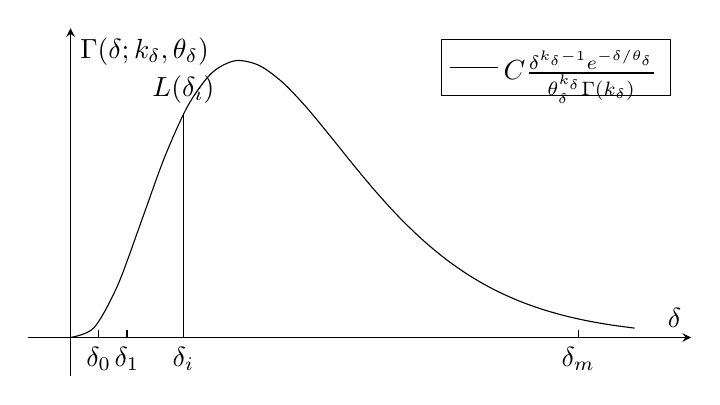
\begin{tikzpicture}[ declare function={gamma(\z)=
    (2.506628274631*sqrt(1/\z) + 0.20888568*(1/\z)^(1.5) + 0.00870357*(1/\z)^(2.5) - (174.2106599*(1/\z)^(3.5))/25920 - (715.6423511*(1/\z)^(4.5))/1244160)*exp((-ln(1/\z)-1)*\z);},
    declare function={gammapdf(\x,\k,\theta) = \x^(\k-1)*exp(-\x/\theta) / (\theta^\k*gamma(\k+1)/\k);}
]
        \begin{axis} [
        width=10cm,height=6cm,
             xmin=-1.5, xmax=22, ymin=-2.5, ymax=20,
            % xtick={-0.5,...,20}, 
            % xtick={$\delta_0$,$\delta_1$},
            % ytick={-2,-1.5,...,2},
            xticklabel style={font=\tiny, xshift=0.5ex},
            yticklabel style={font=\tiny, yshift=0.5ex},
            axis line style={->},
            axis x line=middle,
            axis y line=middle,
            ticks=none,
            xlabel={$\delta$},
            ylabel={$\Gamma(\delta; k_\delta, \theta_\delta)$},
            legend pos=north east
          % legend style={at={(0.17,0.8)},anchor=south west}
        ]
        \addplot [smooth, domain=0:20, black] {160*gammapdf(x,4,2.0)};
        \addplot[-,color=black] coordinates {(4,0) (4,14.5)};
        \node[below] (deltai) at (4,0) {$\delta_i$};
        \node[above] (Ldeltai) at (4,14.5) {$L(\delta_i)$};
        
        \node[below] (delta0) at (1, 0) {$\delta_0$};        
        \node[below] (delta1) at (2, 0) {$\delta_1$};        
        \node[below] (deltak) at (18, 0) {$\delta_m$};        

        \addplot[-,color=black] coordinates {(1,0) (1,0.5)};
        \addplot[-,color=black] coordinates {(2,0) (2,0.5)};
        \addplot[-,color=black] coordinates {(18,0) (18,0.5)};

        \addlegendentry{$C\frac{\delta^{k_\delta-1} e^{-\delta/\theta_\delta} }{\theta_\delta^{k_\delta}\Gamma(k_\delta)}$}
        \end{axis}
    \end{tikzpicture}

\end{document}
        }
        \label{fig:chapter3:sim-pratical-approach-delta}
    }
    \subfloat[]{
    \scalebox{0.8}[0.7] {
        \input{./tikz/sim-pratical-approach-alpha}
        }
        \label{fig:chapter3:sim-pratical-approach-alpha}
    }
    \hfill
    \subfloat[]{
    \scalebox{0.6}[0.7] {
        \documentclass{standalone}
\usepackage{pgfplots}
\pgfplotsset{compat=1.11}
\begin{document}
% Place the TikZ picture in a figure environment.
%\begin{figure}[htb]
% h: here, t: top, b: bottom, p: page of float
%% https://tex.stackexchange.com/questions/39017/how-to-influence-the-position-of-float-environments-like-figure-and-table-in-lat
%% ! indicates that some restrictions should be ignored (discussed later)
%% h indicates that the float is allowed to be placed inline
%% t indicates that the float is allowed to go into a top area
%% b indicates that the float is allowed to go into a bottom area
%% p indicates the the float is allowed to go on a float page or column area

    \begin{tikzpicture}
        \begin{axis} [
        width=12cm,height=5cm,
            xmin=-2, xmax=2, ymin=-0.2, ymax=1.5, 
            % grid=both,
            ylabel={$U(x)$}, xlabel={$x$},
            % xtick={-2,-1.5,...,2}, ytick={-2,-1.5,...,2},
            % xticklabel style={font=\tiny, xshift=0.5ex},
            % yticklabel style={font=\tiny, yshift=0.5ex},
            axis line style={->},
            axis x line=middle,
            axis y line=middle,
            ticks=none
        ]
        
        % \addplot+[line width=1.5pt, color=black, dashed, -, mark=none, domain=-1.3:-1.8] {0};
        %\addplot+[line width=1.5pt,color=black, solid, -, mark=none, domain=-2:-1.3] {0};
        % \addplot+[line width=1.5pt,color=black, solid, -, mark=none, domain=-2:-0.3] {0};
        % \addplot+[line width=1.5pt,color=black, solid, mark=none, domain=-0.3:1] {0};

        % \addplot+[line width=1.5pt,color=black, solid, mark=none, -,domain=1.3:1.8] {+1};

        % \addplot+[line width=1.5pt,color=black, solid, mark=none, -,domain=2:1.3] {+1};
        % \addplot+[line width=1.5pt,color=black, solid, mark=none, -, domain=1.3:0.2] {+1};
        % \addplot+[line width=1.5pt,color=black, solid, mark=none, domain=0.2:-1] {+1};

        % \draw[line width=1.5pt,color=black, solid, mark=none, -] (1, 0) -- (1, 0.2);
        % \draw[line width=1.5pt,color=black, solid, mark=none] (1, 0) -- (1, +1);

        % \draw[line width=1.5pt,color=black, solid, mark=none, -] (-1, +1) -- (-1, +0.2);
        % \draw[line width=1.5pt,color=black, solid, mark=none] (-1, +0.2) -- (-1, 0);

        % \node[below] at (-1.75,-0.05) {$a$};
        % \node[below] at (-1,0) {$b$};
        % \node[below] at (1,0) {$c$};
        % \node[above] at (1,1) {$d$};
        % \node[above] at (1.75,1) {$e$};

        % \node[above] at (-1,1) {$f$};
                
        \addplot+[color=black, solid, mark=none, -,domain=-1:1] {+1};
        \addplot+[color=black, dashed, mark=none] coordinates {(1,1) (1,0)};
        \addplot+[color=black, dashed, mark=none] coordinates {(-1,1) (-1,0)};
        
        \addplot+[color=black, dotted, mark=none] coordinates {(-0.4,1) (-0.4,0)};
        
        \node[below] at (-1,0) {$-\alpha_i$};
        \node[below] at (1,0) {$\alpha_i$};
        \node[below] at (-0.4,0) {$\alpha_0$};
        % \addlegendentry{$U(x)$}

        \end{axis}
    \end{tikzpicture}

\end{document}
        }
        \label{fig:chapter3:sim-pratical-approach-alpha0}
    }
    \subfloat[]{
    % \raisebox{}{}
    \scalebox{0.7}[0.7] {
            \documentclass{standalone}
\usepackage{pgfplots}
\pgfplotsset{compat=1.11}
\begin{document}
% Place the TikZ picture in a figure environment.
%\begin{figure}[htb]
% h: here, t: top, b: bottom, p: page of float
%% https://tex.stackexchange.com/questions/39017/how-to-influence-the-position-of-float-environments-like-figure-and-table-in-lat
%% ! indicates that some restrictions should be ignored (discussed later)
%% h indicates that the float is allowed to be placed inline
%% t indicates that the float is allowed to go into a top area
%% b indicates that the float is allowed to go into a bottom area
%% p indicates the the float is allowed to go on a float page or column area

    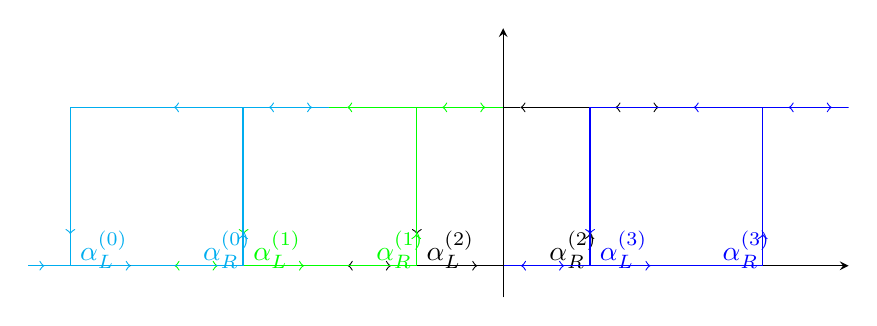
\begin{tikzpicture}
        \begin{axis} [
        width=12cm,height=5cm,
            % xmin=-7.5, xmax=7.5, ymin=-0.5, ymax=1.5, 
            xmin=-5.5, xmax=4.0, ymin=-0.2, ymax=1.5,
            % grid=both,
            ylabel={},
            xlabel=,
            % xtick={-2,-1.5,...,2}, ytick={-2,-1.5,...,2},
            % xticklabel style={font=\tiny, xshift=0.5ex},
            % yticklabel style={font=\tiny, yshift=0.5ex},
            axis line style={->},
            axis x line=middle,
            axis y line=middle,
            ticks=none
        ]
        \addplot+[color=black, dashed, ->, mark=none, domain=-1.3:-1.8] {0};
        \addplot+[color=black, solid, ->, mark=none, domain=-2:-1.3] {0};
        \addplot+[color=black, solid, ->, mark=none, domain=-2:-0.3] {0};
        \addplot+[,color=black, solid, mark=none, domain=-0.3:1] {0};

        \addplot+[color=black, solid, mark=none, ->,domain=1.3:1.8] {+1};

        \addplot+[color=black, solid, mark=none, ->,domain=2:1.3] {+1};
        \addplot+[color=black, solid, mark=none, ->, domain=1.3:0.2] {+1};
        \addplot+[color=black, solid, mark=none, domain=0.2:-1] {+1};

        \draw[color=black, solid, mark=none, ->] (1, 0) -- (1, 0.2);
        \draw[color=black, solid, mark=none] (1, 0) -- (1, +1);

        \draw[color=black, solid, mark=none, ->] (-1, +1) -- (-1, +0.2);
        \draw[color=black, solid, mark=none] (-1, +0.2) -- (-1, 0);

        
        \node[right] at (-1,0.1) {$\alpha^{(2)}_L$};
        \node[left] at (1.2,0.1) {$\alpha^{(2)}_R$};


        %%%%%%%%%%%%%%%%%%%%%%%%%%%%%%%%%%%%%%%%%%%%%%%%%%%%%%
        
        \addplot+[color=blue, dashed, ->, mark=none, domain=-1.3:-1.8][xshift=2.2cm] {0};
        \addplot+[color=blue, solid, ->, mark=none, domain=-2:-1.3][xshift=2.2cm] {0};
        \addplot+[color=blue, solid, ->, mark=none, domain=-2:-0.3][xshift=2.2cm] {0};
        \addplot+[,color=blue, solid, mark=none, domain=-0.3:1][xshift=2.2cm] {0};

        \addplot+[color=blue, solid, mark=none, ->,domain=1.3:1.8][xshift=2.2cm] {+1};

        \addplot+[color=blue, solid, mark=none, ->,domain=2:1.3][xshift=2.2cm] {+1};
        \addplot+[color=blue, solid, mark=none, ->, domain=1.3:0.2][xshift=2.2cm] {+1};
        \addplot+[color=blue, solid, mark=none, domain=0.2:-1][xshift=2.2cm] {+1};

        \draw[color=blue, solid, mark=none, ->][xshift=2.2cm] (1, 0) -- (1, 0.2);
        \draw[color=blue, solid, mark=none][xshift=2.2cm] (1, 0) -- (1, +1);

        \draw[color=blue, solid, mark=none, ->][xshift=2.2cm] (-1, +1) -- (-1, +0.2);
        \draw[color=blue, solid, mark=none][xshift=2.2cm] (-1, +0.2) -- (-1, 0);

        \node[right,color=blue][xshift=2.2cm] at (-1,0.1) {$\alpha^{(3)}_L$};
        \node[left,color=blue][xshift=2.2cm] at (1.2,0.1) {$\alpha^{(3)}_R$};
                

        % %%%%%%%%%%%%%%%%%%%%%%%%%%%%%%%%%%%%%%%%%%%%%%%%%%%
        
        \addplot+[color=green, dashed, ->, mark=none, domain=-1.3:-1.8][xshift=-2.2cm] {0};
        \addplot+[color=green, solid, ->, mark=none, domain=-2:-1.3][xshift=-2.2cm] {0};
        \addplot+[color=green, solid, ->, mark=none, domain=-2:-0.3][xshift=-2.2cm] {0};
        \addplot+[,color=green, solid, mark=none, domain=-0.3:1][xshift=-2.2cm] {0};

        \addplot+[color=green, solid, mark=none, ->,domain=1.3:1.8][xshift=-2.2cm] {+1};

        \addplot+[color=green, solid, mark=none, ->,domain=2:1.3][xshift=-2.2cm] {+1};
        \addplot+[color=green, solid, mark=none, ->, domain=1.3:0.2][xshift=-2.2cm] {+1};
        \addplot+[color=green, solid, mark=none, domain=0.2:-1][xshift=-2.2cm] {+1};

        \draw[color=green, solid, mark=none, ->][xshift=-2.2cm] (1, 0) -- (1, 0.2);
        \draw[color=green, solid, mark=none][xshift=-2.2cm] (1, 0) -- (1, +1);

        \draw[color=green, solid, mark=none, ->][xshift=-2.2cm] (-1, +1) -- (-1, +0.2);
        \draw[color=green, solid, mark=none][xshift=-2.2cm] (-1, +0.2) -- (-1, 0);

        \node[right,color=green][xshift=-2.2cm] at (-1,0.1) {$\alpha^{(1)}_L$};
        \node[left,color=green][xshift=-2.2cm] at (1.2,0.1) {$\alpha^{(1)}_R$};


        %%%%%%%%%%%%%%%%%%%%%%%%%%%%%%%%%%%%%%%%%%%%%%%%%%%%%%
        \addplot+[color=cyan, dashed, ->, mark=none, domain=-1.3:-1.8][xshift=-4.4cm] {0};
        \addplot+[color=cyan, solid, ->, mark=none, domain=-2:-1.3][xshift=-4.4cm] {0};
        \addplot+[color=cyan, solid, ->, mark=none, domain=-2:-0.3][xshift=-4.4cm] {0};
        \addplot+[,color=cyan, solid, mark=none, domain=-0.3:1][xshift=-4.4cm] {0};

        \addplot+[color=cyan, solid, mark=none, ->,domain=1.3:1.8][xshift=-4.4cm] {+1};

        \addplot+[color=cyan, solid, mark=none, ->,domain=2:1.3][xshift=-4.4cm] {+1};
        \addplot+[color=cyan, solid, mark=none, ->, domain=1.3:0.2][xshift=-4.4cm] {+1};
        \addplot+[color=cyan, solid, mark=none, domain=0.2:-1][xshift=-4.4cm] {+1};

        \draw[color=cyan, solid, mark=none, ->][xshift=-4.4cm] (1, 0) -- (1, 0.2);
        \draw[color=cyan, solid, mark=none][xshift=-4.4cm] (1, 0) -- (1, +1);

        \draw[color=cyan, solid, mark=none, ->][xshift=-4.4cm] (-1, +1) -- (-1, +0.2);
        \draw[color=cyan, solid, mark=none][xshift=-4.4cm] (-1, +0.2) -- (-1, 0);

        \node[right,color=cyan][xshift=-4.4cm] at (-1,0.1) {$\alpha^{(0)}_L$};
        \node[left,color=cyan][xshift=-4.4cm] at (1.2,0.1) {$\alpha^{(0)}_R$};

        \end{axis}
    \end{tikzpicture}

\end{document}
    }
    % \scalebox{0.7}[1] {
    %     }
    %  
    \label{fig:chapter3:sim-pratical-approach-relays}
    }    
    % \hfill
    % \subfloat[]{
    % \scalebox{0.8}[0.7] {
    %     \input{./tikz/sim-pratical-approach-beta}
    %     }
    % \label{fig:chapter3:sim-pratical-approach-beta}
    % }        

    % \subfloat[]{
    %   \scalebox{0.8}[0.7] {
    %     \input{./tikz/sim-pratical-approach-beta}
    %     }
    % \label{fig:chapter3:sim-pratical-approach-beta}
    % }        
    
    \caption{Distribution of $\Gamma(\delta; k, \theta)$}
    \label{fig:sim-pratical-approach-delta}
\end{figure}


% First we should choose $\delta$. We fix $\delta_0 > 0, \hat{\delta} > 0, k \in \mathbb{N}$ and consider $\delta_0, \delta_1 = \delta_0 + \hat{\delta}, \ldots, \delta_{k} = \delta_0 + k \hat{\delta}$. So we consider finite sequence of $\delta_i$ with fixed steps. For each $\delta_{i}$ we should find $L(\delta_{i})$. For this purpose we need so-called gamma distribution \citep{wiki:gamma-distribution}. We take one with parameters, $k, \theta, C$. We set $L(\delta_{i}) = C \Gamma_1{(k, \theta)}(\delta_i)$ (see \myfigureref{fig:chapter3:market-real-agents-n-distribution}). 
% Each real agent with strategy corresponding to parameters $\alpha, \alpha_0, n$ s represented
% by $2n$ relays with thresholds $\big(\alpha_0 - n \alpha, \alpha_0 - (n-1) \alpha \big),\big(\alpha_0 - (n-1) \alpha, \alpha_0 - (n-2) \alpha \big), \ldots, \big(\alpha_0 + (n-1) \alpha, \alpha_0 + n \alpha \big)$(at these layers agent buys/sells his stock). At the
% beginning agent have $n$ stocks if $\alpha_0 \ge 0$ and $n-1$ otherwise.

% We choose $\alpha$ also using gamma distribution $\Gamma_2$ (see \myfigureref{fig:chapter3:market-real-agents-alpha-distribution}). $\alpha_0$ we choose using the uniform distribution between $-\alpha$ and $\alpha$. $n$ we find as a root of the equation 

% \begin{equation}\label{eqn:chapter3:root-of-real-agents-n}
%     \delta = \frac{e^{-\alpha}(1-e^{-\alpha n})}{1-e^{-\alpha}}
% \end{equation}

\subsection{Real agent D}
We choose parameter $\beta_i$ (see \myfigref{fig:chapter3:strategy-illustration}, we set $\beta_i = \beta_R = \beta_L$ for convenience.) (when price rises/drops $\beta_i$ points we buy/sell) and decide whether agents have stock at the very beginning. We consider sequence $\beta_i$ with fixed step. We also fix gamma distribution $\Gamma_3$ (see \myfigureref{fig:chapter3:sim-pratical-approach-beta,fig:chapter3:market-virtual-agents-d-distribution}) with some parameters and multiply it by number $B$. We want the amount of stocks for \textit{agents N} and \textit{agents D} keeps the following equation,
$$\sum_{\alpha, \delta_i} n(\alpha, \delta_i) L(\delta_i) = \sum_{i} D_{\textbf{1}}(\beta_i) = B \sum_i \Gamma_3(\beta_i)$$
where $D_{\textbf{1}}(\beta_i)$ is number of agents D corresponded to $\beta_i$ with stock at the very beginning. We also assume that $D_{\textbf{0}}(\beta_i) = D_{\textbf{1}}(\beta_i)$ where $D_{\textbf{0}}(\beta_i)$ is the number of agents D corresponded to $\beta_i$ without stock at the very beginning.

\begin{remark}
\begin{enumerate}
\item Why should we choose gamma distribution? \\
      The probability density function of gamma distribution is in the first quadrant, and it's continuous.
    
    \item Why should we assume that the amount of wealth belonged to people is followed by gamma distribution? \\
    According to \citep{wiki:pareto-distribution}, it makes sense that only a few people possess a large volume of wealth in reality. And we can tune the shape of the gamma distribution to approximate the Pareto distribution.
    
% \item Why should we assume that the width of relay($\alpha$) is followed by gamma distribution ? \\
%     In reality, most people will have the same strategy to react to the change of stock price. (TODO: need reference ?)
\end{enumerate}
\end{remark}

\begin{figure}[htb!]
    % \left
    %\subfloat[]{
        %\raisebox{0px} {
            % \adjustimage{width=\textwidth/2}{
            \subfloat[]{
            \includegraphics[height=3cm,width=\textwidth/2]{market-real-agents-n-distribution}\label{fig:chapter3:market-real-agents-n-distribution}
            }
            \subfloat[]{
            \includegraphics[height=3cm,width=\textwidth/2]{market-virtual-agents-d-distribution}\label{fig:chapter3:market-virtual-agents-d-distribution}
            }
            \hfill
            \subfloat[]{
            \includegraphics[height=3cm,width=\textwidth/2]{market-real-agents-alpha-distribution}\label{fig:chapter3:market-real-agents-alpha-distribution}
            }
    % }
    \caption{\myfigref{fig:chapter3:market-real-agents-n-distribution} shows the distribution of real agents N. \myfigref{fig:chapter3:market-virtual-agents-d-distribution} shows the distribution of virtual agents D. \myfigref{fig:chapter3:market-real-agents-alpha-distribution} shows the distribution of $\alpha$ for each agent. 
    The red dashed curve is \mydelete{sampled from} the density function of gamma \myupdate{distribution}.
    % \myfigref{fig:chapter5:market-virutal-agents-d-distribution} shows the distribution of virtual agents D
    }
    \label{fig:chapter3:agents-distribution}
\end{figure}
% agents takes part in the markets
\begin{figure}[htb!]
    \centering
    \subfloat[]{
    \includegraphics[height=8cm,width=\textwidth]{market-participanted-agents}
    }
    \caption{The detailed inspections of all agents taking part in the market during a simulation. It shows that agents N, agents D and agents E participated at each time step and indicates our market model doesn't degrade to \citep{dima2014}'s model \myupdate{which only contains agents D and agents E.}}
    \label{fig:chapter3:market-participanted-agents}
\end{figure}
% \mytodo{https://en.wikipedia.org/wiki/Pareto_distribution} \\ 
% \mytodo{https://en.wikipedia.org/wiki/Pareto_distribution} \\
% \mytodo{https://en.wikipedia.org/wiki/Lorenz_curve} \\

%%%%%%%%%%%%%%%%%%%%%%%%%%%%%%%%%%%%%%%%%%%%%%%%%%%%%%%%%%
% \mytodo{maybe we need change to exponential distribution} 
